\documentclass[tikz,border=8pt]{standalone}
% Shared look for every TikZ diagram. Load with % Shared look for every TikZ diagram. Load with % Shared look for every TikZ diagram. Load with \input{../../tools/tikz-style.tex}
\usepackage[T1]{fontenc}
\usepackage{lmodern}
\renewcommand{\sfdefault}{lmr}  % diagrams use the same serif as the text
\usetikzlibrary{arrows.meta, positioning, shapes.geometric, calc, fit, backgrounds}
\definecolor{cblue}{HTML}{4C78A8}
\definecolor{corange}{HTML}{F58518}
\definecolor{cgreen}{HTML}{54A24B}
\definecolor{cred}{HTML}{E45756}
\definecolor{cpurple}{HTML}{B279A2}
\definecolor{cgrey}{HTML}{6B6B6B}
\tikzset{
  every picture/.style={font=\sffamily, line width=1.2pt},
  box/.style={draw=#1, fill=#1!12, rounded corners=4pt, align=center, inner sep=7pt, minimum height=1.1cm},
  box/.default=cgrey,
  arrow/.style={-{Stealth[length=3mm]}, draw=cgrey, line width=1.4pt},
  title/.style={font=\sffamily\bfseries\Large},
  note/.style={font=\sffamily\small, text=cgrey, align=center},
}
\AtBeginDocument{\hyphenpenalty=10000 \exhyphenpenalty=10000}

\usepackage[T1]{fontenc}
\usepackage{lmodern}
\renewcommand{\sfdefault}{lmr}  % diagrams use the same serif as the text
\usetikzlibrary{arrows.meta, positioning, shapes.geometric, calc, fit, backgrounds}
\definecolor{cblue}{HTML}{4C78A8}
\definecolor{corange}{HTML}{F58518}
\definecolor{cgreen}{HTML}{54A24B}
\definecolor{cred}{HTML}{E45756}
\definecolor{cpurple}{HTML}{B279A2}
\definecolor{cgrey}{HTML}{6B6B6B}
\tikzset{
  every picture/.style={font=\sffamily, line width=1.2pt},
  box/.style={draw=#1, fill=#1!12, rounded corners=4pt, align=center, inner sep=7pt, minimum height=1.1cm},
  box/.default=cgrey,
  arrow/.style={-{Stealth[length=3mm]}, draw=cgrey, line width=1.4pt},
  title/.style={font=\sffamily\bfseries\Large},
  note/.style={font=\sffamily\small, text=cgrey, align=center},
}
\AtBeginDocument{\hyphenpenalty=10000 \exhyphenpenalty=10000}

\usepackage[T1]{fontenc}
\usepackage{lmodern}
\renewcommand{\sfdefault}{lmr}  % diagrams use the same serif as the text
\usetikzlibrary{arrows.meta, positioning, shapes.geometric, calc, fit, backgrounds}
\definecolor{cblue}{HTML}{4C78A8}
\definecolor{corange}{HTML}{F58518}
\definecolor{cgreen}{HTML}{54A24B}
\definecolor{cred}{HTML}{E45756}
\definecolor{cpurple}{HTML}{B279A2}
\definecolor{cgrey}{HTML}{6B6B6B}
\tikzset{
  every picture/.style={font=\sffamily, line width=1.2pt},
  box/.style={draw=#1, fill=#1!12, rounded corners=4pt, align=center, inner sep=7pt, minimum height=1.1cm},
  box/.default=cgrey,
  arrow/.style={-{Stealth[length=3mm]}, draw=cgrey, line width=1.4pt},
  title/.style={font=\sffamily\bfseries\Large},
  note/.style={font=\sffamily\small, text=cgrey, align=center},
}
\AtBeginDocument{\hyphenpenalty=10000 \exhyphenpenalty=10000}

\begin{document}
% The Notebook's five small models (data/shapes.csv): each layer with the shape it hands on. A 3D shape
% (batch, time steps, values) means one output per time step; a 2D shape means one output per observation.
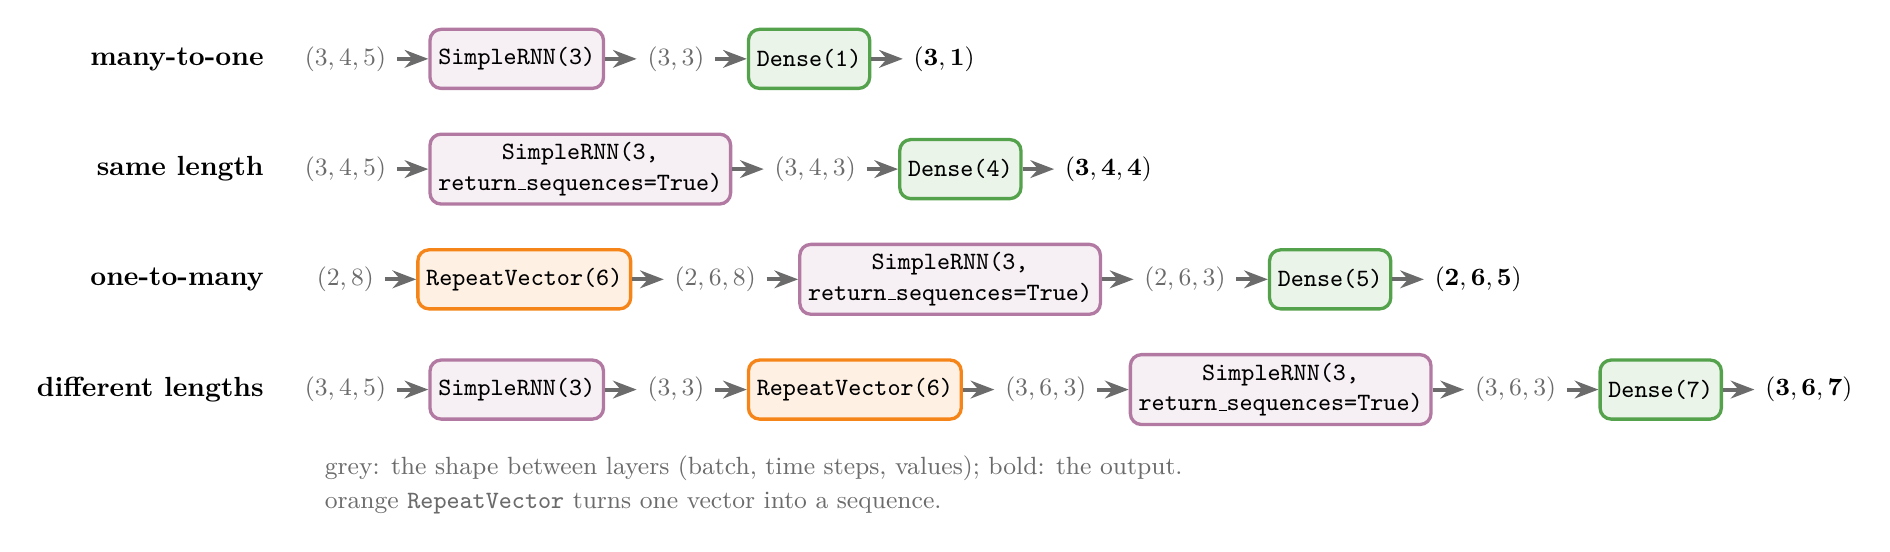
\begin{tikzpicture}[l/.style={box=#1, align=center, minimum height=0.75cm, inner sep=3pt, font=\sffamily\small},
                    s/.style={font=\sffamily\small, text=cgrey}, x=1cm, y=1cm]
  \newcommand{\row}[3]{\node[font=\sffamily\bfseries, anchor=east] at (-0.3, #1) {#2};}
  % many-to-one
  \row{0}{many-to-one}{}
  \node[s] (a0) at (0.6, 0) {$(3, 4, 5)$};
  \node[l=cpurple, right=0.4cm of a0] (a1) {\texttt{SimpleRNN(3)}};
  \node[s, right=0.4cm of a1] (a2) {$(3, 3)$};
  \node[l=cgreen, right=0.4cm of a2] (a3) {\texttt{Dense(1)}};
  \node[s, right=0.4cm of a3, text=black] (a4) {$\mathbf{(3, 1)}$};
  \foreach \u/\v in {a0/a1, a1/a2, a2/a3, a3/a4} \draw[arrow] (\u) -- (\v);
  % many-to-many same
  \row{-1.4}{same length}{}
  \node[s] (b0) at (0.6, -1.4) {$(3, 4, 5)$};
  \node[l=cpurple, right=0.4cm of b0] (b1) {\texttt{SimpleRNN(3,}\\\texttt{return\_sequences=True)}};
  \node[s, right=0.4cm of b1] (b2) {$(3, 4, 3)$};
  \node[l=cgreen, right=0.4cm of b2] (b3) {\texttt{Dense(4)}};
  \node[s, right=0.4cm of b3, text=black] (b4) {$\mathbf{(3, 4, 4)}$};
  \foreach \u/\v in {b0/b1, b1/b2, b2/b3, b3/b4} \draw[arrow] (\u) -- (\v);
  % one-to-many
  \row{-2.8}{one-to-many}{}
  \node[s] (c0) at (0.6, -2.8) {$(2, 8)$};
  \node[l=corange, right=0.4cm of c0] (c1) {\texttt{RepeatVector(6)}};
  \node[s, right=0.4cm of c1] (c2) {$(2, 6, 8)$};
  \node[l=cpurple, right=0.4cm of c2] (c3) {\texttt{SimpleRNN(3,}\\\texttt{return\_sequences=True)}};
  \node[s, right=0.4cm of c3] (c4) {$(2, 6, 3)$};
  \node[l=cgreen, right=0.4cm of c4] (c5) {\texttt{Dense(5)}};
  \node[s, right=0.4cm of c5, text=black] (c6) {$\mathbf{(2, 6, 5)}$};
  \foreach \u/\v in {c0/c1, c1/c2, c2/c3, c3/c4, c4/c5, c5/c6} \draw[arrow] (\u) -- (\v);
  % encoder-decoder
  \row{-4.2}{different lengths}{}
  \node[s] (d0) at (0.6, -4.2) {$(3, 4, 5)$};
  \node[l=cpurple, right=0.4cm of d0] (d1) {\texttt{SimpleRNN(3)}};
  \node[s, right=0.4cm of d1] (d2) {$(3, 3)$};
  \node[l=corange, right=0.4cm of d2] (d3) {\texttt{RepeatVector(6)}};
  \node[s, right=0.4cm of d3] (d4) {$(3, 6, 3)$};
  \node[l=cpurple, right=0.4cm of d4] (d5) {\texttt{SimpleRNN(3,}\\\texttt{return\_sequences=True)}};
  \node[s, right=0.4cm of d5] (d6) {$(3, 6, 3)$};
  \node[l=cgreen, right=0.4cm of d6] (d7) {\texttt{Dense(7)}};
  \node[s, right=0.4cm of d7, text=black] (d8) {$\mathbf{(3, 6, 7)}$};
  \foreach \u/\v in {d0/d1, d1/d2, d2/d3, d3/d4, d4/d5, d5/d6, d6/d7, d7/d8} \draw[arrow] (\u) -- (\v);
  \node[note, anchor=west] at (0.2, -5.2) {grey: the shape between layers (batch, time steps, values); bold: the output.};
  \node[note, anchor=west] at (0.2, -5.65) {orange \texttt{RepeatVector} turns one vector into a sequence.};
\end{tikzpicture}
\end{document}
